\begin{apendicesenv}

\partapendices

\chapter{Módulo matemático 0}
\label{apd:kmeans}

Um módulo matemático implementado no ``Empurrando Juntos'' é baseado no algoritmo k-Means, apresentado no Capítulo \ref{cap:clusterizacao}. 

No ``Empurrando Juntos'' a entrada para os \textit{clusters} é a combinação entre participante,  
comentário e o voto. Essa combinação gera uma entrada de N dimensões para N comentários.
Frequentemente antes de medir a similaridade entre os objetos é necessário
reduzir a dimensionalidade, isso acontece, pois para espaços de alta dimensão as distâncias euclidianas
tendem a inflar. Reduzir a dimensionalidade pode aliviar esse problema e diminuir o tempo de cálculo.
Um dos métodos mais utilizados para realizar essa redução é a Análise de 
Componentes Principais (PCA, do inglês) \cite{han2011data, sklearn}.

\citeonline{han2011data} afirmam que o PCA cria $k$ vetores ortogonais que possuem o mesmo significado que o conjunto
de vetores inicial, porém trata-se de um conjunto menor. Para aplicação desse método são realizados basicamente quatro procedimentos.

\begin{enumerate}
 \item Normalizar os dados de entrada, para que eles estejam dentro da mesma variação;
 \item Computar $k$ vetores ortonormais, ou seja, vetores de magnitude 1, nos quais cada ponto é perpendicular aos outros;
  \subitem Esses vetores são chamados de componentes principais.
 \item Ordenar decrescentemente os componentes principais pela significância;
 \item Remover os componentes ``fracos'', ou seja, aqueles com pouca variância.
\end{enumerate}

No final dos quatro procedimentos, os componentes principais restantes são uma boa aproximação dos dados originais \cite{han2011data}.
Além disso, foi aplicada uma técnica analítica para a definição do melhor valor para $k$, conhecida como Coeficiente de Silhueta \cite{sklearn}.

Essa técnica tem por objetivo combinar a avaliação de coesão e separação dos \textit{clusters} por meio do cálculo de um coeficiente (o de silhueta) que 
varia de -1 a 1 e é dado pela fórmula \ref{eq:coeficiente} \cite{tan2013data}.

\begin{equation} \label{eq:coeficiente}
  s_{i} = \frac{(b_{i} - a_{i})}{max(a_{i}, b_{i})} \mbox{, onde:}
\end{equation}

{\addtolength{\leftskip}{8mm}
    i é o objeto do \textit{cluster} que está sendo analisado
    
    $a_{i}$ é a média da distância entre o objeto e todos os objetos do seu \textit{cluster}
    
    $b_{i}$ é o valor mínimo da distância entre o objeto e os demais \textit{clusters}. 
    
	  \footnotesize \indent \indent A distância entre o objeto e outro \textit{cluster} é média das distâncias entre o objeto \\ \indent \indent e todos os objetos do outro \textit{cluster}.
}

Um coeficiente negativo representa que o elemento está no \textit{cluster} errado, pois isso significa que a distância entre o objeto e outro \textit{cluster} 
é menor que a distância entre o objeto e os objetos de seu \textit{cluster}. O valor ``zero'' representa que o elemento está próximo da ``borda'' do \textit{cluster}, ou seja,
a distância entre o objeto e outros \textit{clusters} e entre o objeto e os objetos de seu \textit{cluster} é a mesma. E por fim, quanto mais próximo do valor 1, melhor
está a distribuição dos \textit{clusters}, pois significa que o valor de $a_i$ é menor que o valor de $b_i$.

Dessa forma, com a escolha de um intervalo de valores para $k$, como sugerido por \citeonline{han2011data} e \citeonline{sklearn}, é possível testar os valores 
para o coeficiente de silhueta e escolher o melhor valor de $k$ dentro do intervalo. 

\begin{figure}[bt!]
\centering
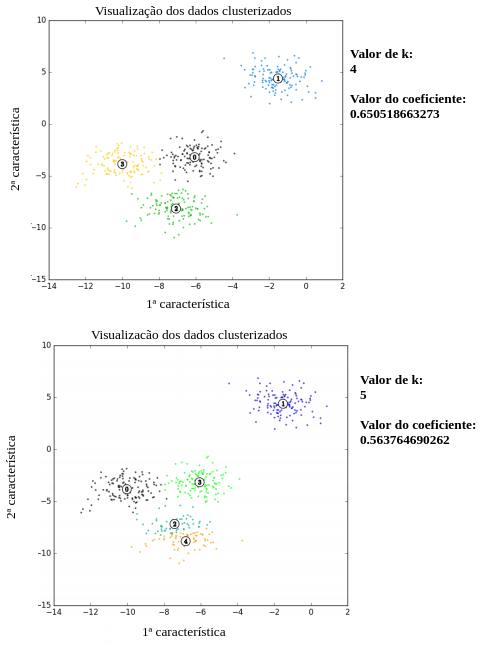
\includegraphics[scale=1]{figuras/exemplo_silhueta.png}
\caption{Formação de \textit{clusters} utilizando K-means e seus coeficientes de silhueta. Adaptado de \citeonline{sklearn}}
\label{fig:exemplo_silhueta}
\end{figure}

\vfill
\pagebreak
Na Figura \ref{fig:exemplo_silhueta} é apresentado um exemplo visual de \textit{clusters} com diferentes valores
de $k$ e seus coeficientes de silhueta.

Os métodos e técnicas apresentados fazem parte do algoritmo implementado no módulo de clusterização da plataforma 
e possuem um objetivo específico. 

\begin{figure}[h!]
\centering
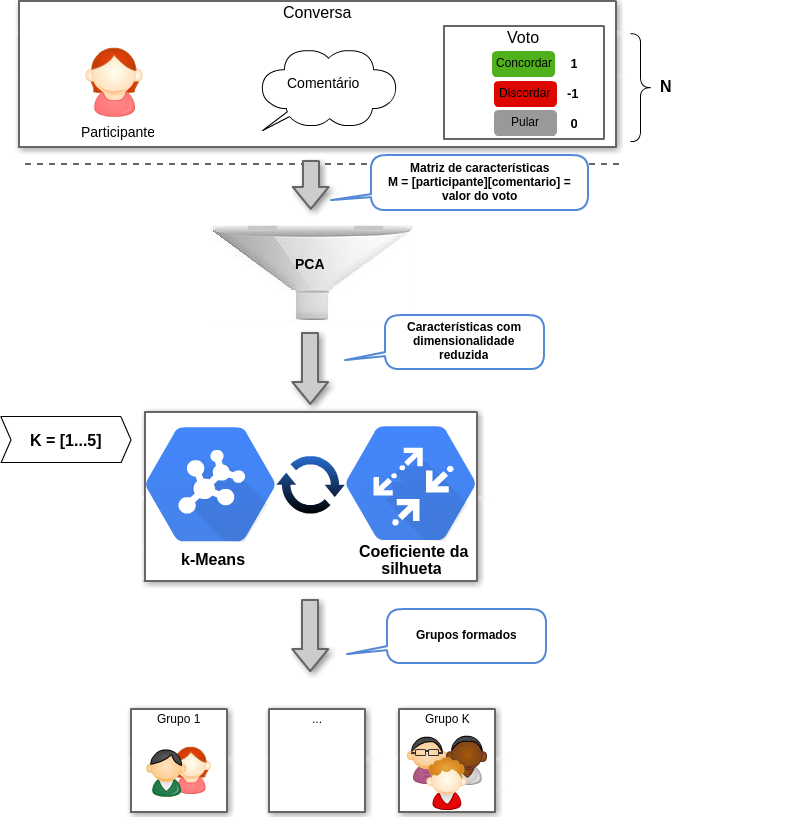
\includegraphics[scale=0.7]{figuras/resumo_clusterizao_ej.png}
\caption{Fluxo de clusterização do ``Empurrando Juntos''}
\label{fig:resumo_clusterizao_ej}
\end{figure}

Quando o usuário cria uma conversa e outros participantes realizam comentários, para cada usuário é permitido realizar votos nesse comentários.
Atualmente, a ideia é que o voto seja concordar, discordar ou pular. 

\vfill 
\pagebreak
A cada novo voto o fluxo apresentado na Figura \ref{fig:resumo_clusterizao_ej} é
realizado. Para cada conversa, os N votos realizados nos N comentários são a entrada para o módulo de clusterização, 
gerando uma entrada de dimensão N. A partir disso, é aplicada a técnica de PCA para que
essa dimensionalidade seja reduzida. Com os dados em duas dimensões, é aplicada
a técnica k-Means, para obtenção da disposição dos grupos de pessoas. O uso da técnica é
feito em ciclos para a descoberta do melhor valor de $k$ por meio do cálculo do Coeficiente da silhueta.
No final dos ciclos, a saída do fluxo são formados os grupos de pessoas com opiniões semelhantes.
% 
% O módulo de serviço, resultado deste trabalho, estabelece comunicação direta com este módulo de clusterização. 
% No módulo de serviço estão contidas todas as entidades que estabelecem os dados de entrada para a formação dos \textit{clusters}.

\end{apendicesenv}
